% Options for packages loaded elsewhere
\PassOptionsToPackage{unicode}{hyperref}
\PassOptionsToPackage{hyphens}{url}
%
\documentclass[
  a4paper,
  onecolumn,
  oneside]{book}

\usepackage{amsmath,amssymb}
\usepackage{lmodern}
\usepackage{iftex}
\ifPDFTeX
  \usepackage[T1]{fontenc}
  \usepackage[utf8]{inputenc}
  \usepackage{textcomp} % provide euro and other symbols
\else % if luatex or xetex
  \usepackage{unicode-math}
  \defaultfontfeatures{Scale=MatchLowercase}
  \defaultfontfeatures[\rmfamily]{Ligatures=TeX,Scale=1}
\fi
% Use upquote if available, for straight quotes in verbatim environments
\IfFileExists{upquote.sty}{\usepackage{upquote}}{}
\IfFileExists{microtype.sty}{% use microtype if available
  \usepackage[]{microtype}
  \UseMicrotypeSet[protrusion]{basicmath} % disable protrusion for tt fonts
}{}
\makeatletter
\@ifundefined{KOMAClassName}{% if non-KOMA class
  \IfFileExists{parskip.sty}{%
    \usepackage{parskip}
  }{% else
    \setlength{\parindent}{0pt}
    \setlength{\parskip}{6pt plus 2pt minus 1pt}}
}{% if KOMA class
  \KOMAoptions{parskip=half}}
\makeatother
\usepackage{xcolor}
\setlength{\emergencystretch}{3em} % prevent overfull lines
\setcounter{secnumdepth}{5}
% Make \paragraph and \subparagraph free-standing
\ifx\paragraph\undefined\else
  \let\oldparagraph\paragraph
  \renewcommand{\paragraph}[1]{\oldparagraph{#1}\mbox{}}
\fi
\ifx\subparagraph\undefined\else
  \let\oldsubparagraph\subparagraph
  \renewcommand{\subparagraph}[1]{\oldsubparagraph{#1}\mbox{}}
\fi


\providecommand{\tightlist}{%
  \setlength{\itemsep}{0pt}\setlength{\parskip}{0pt}}\usepackage{longtable,booktabs,array}
\usepackage{calc} % for calculating minipage widths
% Correct order of tables after \paragraph or \subparagraph
\usepackage{etoolbox}
\makeatletter
\patchcmd\longtable{\par}{\if@noskipsec\mbox{}\fi\par}{}{}
\makeatother
% Allow footnotes in longtable head/foot
\IfFileExists{footnotehyper.sty}{\usepackage{footnotehyper}}{\usepackage{footnote}}
\makesavenoteenv{longtable}
\usepackage{graphicx}
\makeatletter
\def\maxwidth{\ifdim\Gin@nat@width>\linewidth\linewidth\else\Gin@nat@width\fi}
\def\maxheight{\ifdim\Gin@nat@height>\textheight\textheight\else\Gin@nat@height\fi}
\makeatother
% Scale images if necessary, so that they will not overflow the page
% margins by default, and it is still possible to overwrite the defaults
% using explicit options in \includegraphics[width, height, ...]{}
\setkeys{Gin}{width=\maxwidth,height=\maxheight,keepaspectratio}
% Set default figure placement to htbp
\makeatletter
\def\fps@figure{htbp}
\makeatother
\newlength{\cslhangindent}
\setlength{\cslhangindent}{1.5em}
\newlength{\csllabelwidth}
\setlength{\csllabelwidth}{3em}
\newlength{\cslentryspacingunit} % times entry-spacing
\setlength{\cslentryspacingunit}{\parskip}
\newenvironment{CSLReferences}[2] % #1 hanging-ident, #2 entry spacing
 {% don't indent paragraphs
  \setlength{\parindent}{0pt}
  % turn on hanging indent if param 1 is 1
  \ifodd #1
  \let\oldpar\par
  \def\par{\hangindent=\cslhangindent\oldpar}
  \fi
  % set entry spacing
  \setlength{\parskip}{#2\cslentryspacingunit}
 }%
 {}
\usepackage{calc}
\newcommand{\CSLBlock}[1]{#1\hfill\break}
\newcommand{\CSLLeftMargin}[1]{\parbox[t]{\csllabelwidth}{#1}}
\newcommand{\CSLRightInline}[1]{\parbox[t]{\linewidth - \csllabelwidth}{#1}\break}
\newcommand{\CSLIndent}[1]{\hspace{\cslhangindent}#1}

\makeatletter
\@ifpackageloaded{tcolorbox}{}{\usepackage[many]{tcolorbox}}
\@ifpackageloaded{fontawesome5}{}{\usepackage{fontawesome5}}
\definecolor{quarto-callout-color}{HTML}{909090}
\definecolor{quarto-callout-note-color}{HTML}{0758E5}
\definecolor{quarto-callout-important-color}{HTML}{CC1914}
\definecolor{quarto-callout-warning-color}{HTML}{EB9113}
\definecolor{quarto-callout-tip-color}{HTML}{00A047}
\definecolor{quarto-callout-caution-color}{HTML}{FC5300}
\definecolor{quarto-callout-color-frame}{HTML}{acacac}
\definecolor{quarto-callout-note-color-frame}{HTML}{4582ec}
\definecolor{quarto-callout-important-color-frame}{HTML}{d9534f}
\definecolor{quarto-callout-warning-color-frame}{HTML}{f0ad4e}
\definecolor{quarto-callout-tip-color-frame}{HTML}{02b875}
\definecolor{quarto-callout-caution-color-frame}{HTML}{fd7e14}
\makeatother
\makeatletter
\makeatother
\makeatletter
\@ifpackageloaded{bookmark}{}{\usepackage{bookmark}}
\makeatother
\makeatletter
\@ifpackageloaded{caption}{}{\usepackage{caption}}
\AtBeginDocument{%
\ifdefined\contentsname
  \renewcommand*\contentsname{Table of contents}
\else
  \newcommand\contentsname{Table of contents}
\fi
\ifdefined\listfigurename
  \renewcommand*\listfigurename{List of Figures}
\else
  \newcommand\listfigurename{List of Figures}
\fi
\ifdefined\listtablename
  \renewcommand*\listtablename{List of Tables}
\else
  \newcommand\listtablename{List of Tables}
\fi
\ifdefined\figurename
  \renewcommand*\figurename{Figure}
\else
  \newcommand\figurename{Figure}
\fi
\ifdefined\tablename
  \renewcommand*\tablename{Table}
\else
  \newcommand\tablename{Table}
\fi
}
\@ifpackageloaded{float}{}{\usepackage{float}}
\floatstyle{ruled}
\@ifundefined{c@chapter}{\newfloat{codelisting}{h}{lop}}{\newfloat{codelisting}{h}{lop}[chapter]}
\floatname{codelisting}{Listing}
\newcommand*\listoflistings{\listof{codelisting}{List of Listings}}
\makeatother
\makeatletter
\@ifpackageloaded{caption}{}{\usepackage{caption}}
\@ifpackageloaded{subcaption}{}{\usepackage{subcaption}}
\makeatother
\makeatletter
\@ifpackageloaded{tcolorbox}{}{\usepackage[many]{tcolorbox}}
\makeatother
\makeatletter
\@ifundefined{shadecolor}{\definecolor{shadecolor}{rgb}{.97, .97, .97}}
\makeatother
\makeatletter
\@ifpackageloaded{sidenotes}{}{\usepackage{sidenotes}}
\@ifpackageloaded{marginnote}{}{\usepackage{marginnote}}
\makeatother
\makeatletter
\makeatother
\ifLuaTeX
  \usepackage{selnolig}  % disable illegal ligatures
\fi
\IfFileExists{bookmark.sty}{\usepackage{bookmark}}{\usepackage{hyperref}}
\IfFileExists{xurl.sty}{\usepackage{xurl}}{} % add URL line breaks if available
\urlstyle{same} % disable monospaced font for URLs
\hypersetup{
  pdftitle={Site Mapping Guide},
  pdfauthor={International Organisation for Migration},
  hidelinks,
  pdfcreator={LaTeX via pandoc}}

\title{Site Mapping Guide}
\author{International Organisation for Migration}
\date{}

\begin{document}
\frontmatter
\maketitle
\ifdefined\Shaded\renewenvironment{Shaded}{\begin{tcolorbox}[enhanced, interior hidden, sharp corners, boxrule=0pt, borderline west={3pt}{0pt}{shadecolor}, frame hidden, breakable]}{\end{tcolorbox}}\fi

\renewcommand*\contentsname{Table of contents}
{
\setcounter{tocdepth}{2}
\tableofcontents
}
\listoffigures
\mainmatter
\bookmarksetup{startatroot}

\hypertarget{introduction}{%
\chapter*{Introduction}\label{introduction}}
\addcontentsline{toc}{chapter}{Introduction}

\markboth{Introduction}{Introduction}

Welcome to \emph{SiteMapping.Guide}, an online guidance for the
production of site maps in humanitarian response. Site maps are a key
resource at all stages of a camp lifecycle; from the site planning of
empty or partially settled land; the coordination and management of
services on a site; the development and improvement of a sites'
infrastructure; to the site closure/handover/decommissioning stage.

The aim of this guidance is fourfold:

\begin{enumerate}
\def\labelenumi{\arabic{enumi}.}
\item
  \textbf{Broaden the development of site maps to more humanitarian
  actors} and profiles, mainstreaming the skills required and reducing
  reliance on a limited pool of specialized profiles.
\item
  \textbf{Increase the speed at which site maps are developed.} The
  shorter the lead time for creating site maps, the more useful they are
  for planning activities and coordinating partners in site, especially
  in sudden onset contexts.
\item
  \textbf{Scale the availability of site maps} to increase their benefit
  to reponses in a wider number of sites as well as in a wider number of
  countries.
\item
  Encourage the creation of \textbf{consistent site map products}, in
  terms of visuals, quality and process that are affected
  population-centric and that adhere to data responsibility and
  safeguarding standards.
\end{enumerate}

\begin{tcolorbox}[enhanced jigsaw, opacitybacktitle=0.6, colbacktitle=quarto-callout-warning-color!10!white, breakable, coltitle=black, title=\textcolor{quarto-callout-warning-color}{\faExclamationTriangle}\hspace{0.5em}{Warning}, toprule=.15mm, bottomrule=.15mm, colback=white, left=2mm, toptitle=1mm, bottomtitle=1mm, arc=.35mm, colframe=quarto-callout-warning-color-frame, titlerule=0mm, opacityback=0, rightrule=.15mm, leftrule=.75mm]

This guidance is in draft-stage, much of the content is missing and its
structure may be subject to change.

\end{tcolorbox}

The Site Mapping Guide provides a full step-by-step workflow to develop
site maps. It also outlines key considerations and data protection risks
associated with the management of drone captured imagery, as well as the
responsible dissemination of related information products produced in
the process.

This guide presents two different approaches to developing site maps.
The first approach uses existing satellite imagery and the second uses
drones to capture aerial imagery of sites when and where satellite
imagery is not available or not suitable.

\begin{figure}

{\centering \includegraphics[width=1\textwidth,height=\textheight]{./images/workflow.png}

}

\caption{\label{fig-workflow}The Site Mapping Workflow \emph{Source:
IOM}}

\end{figure}

\hypertarget{what-is-a-site-map}{%
\section*{What is a Site Map?}\label{what-is-a-site-map}}
\addcontentsline{toc}{section}{What is a Site Map?}

\markright{What is a Site Map?}

While no strict definition of a site map exists, this guidance considers
site maps to be physical or electronic maps of IDP displacement sites
that use imagery (aerial or satellite), along with the tracing and
labelling of infrastructure (current or planned) as a tool for planning,
coordination and risk analysis.

\begin{tcolorbox}[enhanced jigsaw, opacitybacktitle=0.6, colbacktitle=quarto-callout-note-color!10!white, breakable, coltitle=black, title=\textcolor{quarto-callout-note-color}{\faInfo}\hspace{0.5em}{Note}, toprule=.15mm, bottomrule=.15mm, colback=white, left=2mm, toptitle=1mm, bottomtitle=1mm, arc=.35mm, colframe=quarto-callout-note-color-frame, titlerule=0mm, opacityback=0, rightrule=.15mm, leftrule=.75mm]

Infographics or maps, which focus on needs or activity/output-level
indicators are, for the purpose of this document, considered as Site
Profiles rather than Site Maps and are beyond the scope of this guide.

\end{tcolorbox}

\hypertarget{audience}{%
\section*{Audience}\label{audience}}
\addcontentsline{toc}{section}{Audience}

\markright{Audience}

This guide is for any Camp Coordination Camp Management, Shelter, or
assessment actor, working in humanitarian contexts, requiring site maps
to do site planning, camp coordination or risk analysis and working at
either agency or inter-agency level.

While some prior knowledge of GIS software is beneficial for those who
plan to use this guide, it is not a prerequisite. We hope that the steps
documented in the below chapters are sufficient in detail and clarity
for first-time users and will accompany new and experienced site mappers
through the process of making site maps, from creating and visualising
spatial data to exporting and disseminating standardized site maps.

While the guidance is relevant for all humanitarian staff, section that
are specifc to IOM can be found in blue boxes like the following:

\begin{tcolorbox}[enhanced jigsaw, opacitybacktitle=0.6, colbacktitle=quarto-callout-note-color!10!white, breakable, coltitle=black, title=\textcolor{quarto-callout-note-color}{\faInfo}\hspace{0.5em}{Note for IOM staff}, toprule=.15mm, bottomrule=.15mm, colback=white, left=2mm, toptitle=1mm, bottomtitle=1mm, arc=.35mm, colframe=quarto-callout-note-color-frame, titlerule=0mm, opacityback=0, rightrule=.15mm, leftrule=.75mm]

Sections in the guidance that are specific to IOM staff will appear in
boxes like this.

\end{tcolorbox}

\hypertarget{when-and-how-to-use-them}{%
\section*{When and how to use them}\label{when-and-how-to-use-them}}
\addcontentsline{toc}{section}{When and how to use them}

\markright{When and how to use them}

Site maps can illustrate camp settings in both sudden-onset disasters as
well as protracted emergencies. They can be used to support the
following activities:

\begin{itemize}
\item
  \textbf{Site planning} during sudden-onset emergencies or protracted
  crises.
\item
  \textbf{Site improvements} - using site maps to plan improvements to
  infrastructure and site layout for disability and inclusion, GBV and
  fire hazard risk mitigation.
\item
  \textbf{Site-level camp coordination} amongst service providers and
  ensuring coordination in the establishment of essential site
  infrastructure and camp services.
\item
  CCCM coordination at the Cluster-level.
\item
  GBV/ Protection \textbf{Safety Audits} conducted through direct
  observation, key informant interviews, focus group discussions.
\end{itemize}

\begin{figure}

{\centering 

\href{images/wau1.jpg}{\includegraphics{./images/wau1.jpg}}

}

\caption{Rehabilation of Wau PoC site \emph{Source: IOM}}

\end{figure}

\hypertarget{acknowledgments}{%
\section*{Acknowledgments}\label{acknowledgments}}
\addcontentsline{toc}{section}{Acknowledgments}

\markright{Acknowledgments}

This guide was developed by IOM, with considerable inputs, support and
feedback by many experts in fields such as site planning, GIS, CCCM and
GBV. Financial support for this guide was generously provided by United
States Bureau of Population, Refugees, and Migration (BPRM) through the
Safe From the Start Initiative. A full list of names of those who
contributed or support to this guide can be found in the
\href{/annexes/acknowledgements.html}{acknowledgements annex}.

\hypertarget{feedback}{%
\section*{Feedback}\label{feedback}}
\addcontentsline{toc}{section}{Feedback}

\markright{Feedback}

Many of the approaches and software/hardware tools are quickly evolving
and improving. As such, we consider this guide to be a living document.
If you have any suggestions on how we can improve this guide, please
reach out to majones@iom.int and bmcdonald@iom.int.

\part{Part 1 - Preparation}

\hypertarget{identifying-requirements}{%
\chapter{Identifying requirements}\label{identifying-requirements}}

Producing site maps requires a significant investment of personnel,
time, software and hardware. In addition to these, the
political/security/conflict context of the area, as well community
acceptance and regulatory framework are factors to consider in whether
or not site maps can be developed in your context and if so, which
approach is most feasible.

Before jumping into \textbf{how} to develop site maps, it is important
to first assess \textbf{if they can or should} be developed:

\begin{enumerate}
\def\labelenumi{\arabic{enumi}.}
\item
  \textbf{Are site maps needed} in your context and what activities or
  decisions will they inform?
\item
  What \textbf{stakeholders} need to be involved, both in the
  development of the site maps (affected population, local and national
  authorities, staff, etc) and in their use (CCCM actors, local
  authorities, etc)? \emph{How will buy in from these stakeholders be
  ensured?}
\item
  \textbf{What is required} to develop site maps in your context?
  Regardless of the chosen approach, the development of site maps
  requires funding, personnel, time, hardware, software, and
  connectivity. A shortcoming on any of these may affect the feasibility
  or timeline of the development of site maps.
\item
  What red-line **contextual challenges*, risks and sensitivities exist
  or may arise during the development of the site maps that could affect
  the overall feasibility or appropriateness of their development?
\end{enumerate}

\hypertarget{stakeholders}{%
\section{Stakeholders}\label{stakeholders}}

Whilst the development of site maps should be approach and context
dependent, typically the following stakeholders will be involved:

\begin{itemize}
\item
  \textbf{Affected population in sites.} These need to be consulted
  before collecting drone-captured imagery to make sure they are
  informed and consent to the activity in order to minimize risks
  associated with this approach and prevent any misunderstandings.
\item
  \textbf{Humanitarian actors.} These can help inform which and how many
  sites need to be mapped. Humanitarian actors, especially those on the
  ground, will also feed into the iteration process of the site maps, in
  order to validate geographic information and keep the maps and the
  underlying data layers up to date.
\item
  \textbf{Authorities.} The authorities are a crucial interlocutor for
  approvals. In addition, their engagement can promote the use of the
  site maps in decision making processes. The participation of
  authorities in the site mapping process will also facilitate the
  handover and long term management of information, expertise and
  equipment, as well as support capacity development initiatives for
  future scenarios.
\item
  \textbf{Legal team.} IOM Legal colleagues will provide any additional
  guidance on data collection, processing and sharing related to your
  specific context and are responsible for providing the final approval
  on the use of drones.
\end{itemize}

\hypertarget{general-requirements}{%
\section{General Requirements}\label{general-requirements}}

Developing site maps typically requires the following:

\hypertarget{personnel}{%
\subsection{Personnel}\label{personnel}}

Staff with relevant skills and expertise. Support staff such as drivers
and procurement support will also be needed. Depending on the number of
sites and how quickly the site maps are needed, the site mapping team
may need to be scaled up.

\hypertarget{context}{%
\subsection{Context}\label{context}}

The security, political and regulatory environment play a large role in
determining the approach to site mapping in a country but also whether
or not the process is feasible at all. Identification of such challenges
and potential risks is best done as early as possible to avoid wasting
resources or to allow sufficient time to mitigate them.

\hypertarget{time}{%
\subsection{Time}\label{time}}

Developing site maps can be a time-intensive process, requiring prior
consultations with various stakeholders, lead-time for procurement of
equipment, travel time for site visits, time for collecting and
processing the imagery, composing the site maps and collaboratively
iterating and updating their content. These are important factors to
consider when looking at the time frame of their intended use.

\hypertarget{funding}{%
\subsection{Funding}\label{funding}}

There are a series of finanical costs involved in the development of
site maps that need to be taken into account. Annex 4 provides a table
with indicative figures for the purpose of costing a site mapping
exercise.

\hypertarget{hardware-and-software}{%
\subsection{Hardware and Software}\label{hardware-and-software}}

\textbf{Hardware requirements} must include: a laptop (with sufficent
processing power, RAM and storage); the drone kit (drone, remote,
batteries etc.); a smartphone (for use as a controller); ground-control
points (printout or spray paint). It is optional but advised to also
have tablets, to support usage of the maps and any connected data
collection exercised.

\textbf{Software requirements} include: QGIS (or similar such as
ArcGIS); WebODM (or similar such as PIX4D); DJI Fly mobile app;
Dronelink mobile app (or similar for flight planning); Avenza Maps (or
similar, for geoPDF usage) \footnote{Where possible free and open source
  software is used in the process, in-line with the
  \href{https://www.un.org/en/content/digital-cooperation-roadmap/}{UN
  Secretary General's Roadmap for Digital Cooperation} An exeption for
  this are the Dronlink app which is commercial and Avenza Maps which is
  free but with paid features.}

\hypertarget{connectivity}{%
\subsection{Connectivity}\label{connectivity}}

In situations of sudden onset disasters, connectivity can be very
challenging and quite often can lead to bottlenecks and delays. While
connectivity requirements vary depending on the chosen approach, a
minimum degree of connectivity should be assumed for the initial
gathering the required geographic information and data layers.

If using satellite imagery sufficent connectivity to download the
imagery is required, or alternatively all map development can be done
remotely with feedback from within country. Connectivity also affects
the UAV imagery workflow as limited connectivity will require the use of
offline tools only and for all processing of the imagery to be done
locally. In areas with good connectivity, the imagery can be transferred
to remote tools and computers for processing, allowing for a higher
degree of remote support.

\hypertarget{deciding-on-an-approach}{%
\chapter{Deciding on an approach}\label{deciding-on-an-approach}}

There are two approaches to making sites maps presented in this guide.
The main differerence between the two is in how aerial imagery is
obtained:

\begin{enumerate}
\def\labelenumi{\arabic{enumi}.}
\tightlist
\item
  Using high-resolution satellite imagery.
\item
  Using drones to capture aerial images of the site.
\end{enumerate}

\begin{figure}

{\centering 

\href{images/droneuseschallenges.png}{\includegraphics[width=0.5\textwidth,height=\textheight]{part1/images/droneuseschallenges.png}}

}

\caption{\label{fig-droneuseschallenges}Uses and challenges of drone use
\emph{Source: ICRC}}

\end{figure}

Each of these approaches have pros and cons and it is important to
evaluate each approach against the following criteria before assessing
which approach to take in your context:\\

\hypertarget{information-needs}{%
\section{Information Needs}\label{information-needs}}

It is important to be clear on what images you want to collect and for
which specific purpose. Consider whether you need only an
image/orthomosaic or whether you are look to create a Digital Elevation
Model, a 3D model, a NDVI index etc. as this will affect your flight
plan. Think about whether there are others applications outside of site
mapping that you are in need of, such as drainage analysis, slope
analysis, landslide risk analysis or vegetation cover analysis. Consider
what area needs to be covered whilst bearing in mind that larger areas
require longer flight times, more storage etc.

You should not be flying the drone above as many areas as possible to
collect as many images as possible and then decide what to do with them.
The data collection must be adequate, relevant and not excessive in
relation to its purpose (only collect data which is needed).

\hypertarget{conflict-and-data-sensitivity}{%
\section{Conflict and Data
Sensitivity}\label{conflict-and-data-sensitivity}}

Due to protection risks, the humanitarian use of drones in conflict
settings is strongly discouraged. The term ``dual-use technology'' is
commonly used to describe a technology with both civilian and military
applications. With the rise of the use of drones for military use, there
is a risk that the use of drones for humanitarian purposes in sites may
be perceived as a security threat by the site population or cause trauma
due to an association of drones with their military uses. In conflict
settings armed actors or authorities are likely to perceive the flying
of drones as both a security and informational risk. This means that the
importation of drone equipment and/ or the request for flight approvals
will likely be denied, or that their use in a site risk being perceived
as a security threat. {[}\^{}footnote{]}

There are \textbf{key considerations to take into account when
collecting, processing and sharing any type of data}. These
considerations determine the degree of sensitivity applied throughout
the data life cycle and include:

\begin{itemize}
\tightlist
\item
  The potential to harm data subjects and others;
\item
  The potential to discriminate;
\item
  The potential to harm IOM staff and individuals representing
  authorized third parties.
\end{itemize}

In addition to the data risks and concerns outlined in the
\href{https://publications.iom.int/books/iom-data-protection-manual}{IOM
Data Protection Manual}, there are additional specific concerns and
risks associated with the use of drones.\footnote{\href{https://publications.iom.int/books/iom-data-protection-manual}{IOM
  Data Protection Manual}}

Once your flight area is identified, a risk-benefit assessment should be
conducted prior to using drones. The assessment will evaluate the risks
and benefits associated with collecting and processing drone captured
imagery and determine whether flying a drone for the collection of
aerial imagery is the best approach in your context.

\hypertarget{data-security-and-responsibility}{%
\section{Data Security and
Responsibility}\label{data-security-and-responsibility}}

The use of drones to capture aerial images for site mapping does not
require the collection of personal data. \textbf{Individuals must not be
identifiable} from captured images. Ensure that the flight settings
(altitude, angle etc.) eliminates or reduces as much as possible the
likelihood that the captured imagery may directly or indirectly identify
an individual. If, by mistake, you collect images in which people can be
identified, you should immediately delete them. However, if the image
taken must really be used, you can either crop the image or blur the
faces of people who could be identified. While collecting the data or
shortly thereafter, check whether any of the images captured contains
sensitive data and therefore should be deleted or otherwise removed
from/made unrecognizable in the image (for example, a group of
individuals that could be identified as part of a specific group, image
of illegal crops or settlement).

\hypertarget{community-engagement}{%
\section{Community Engagement}\label{community-engagement}}

Creating Site Maps requires buy-in from the community in and around the
sites area of interest, in which they are informed of the planned
activity, understand how its planned to be used and why its needed and
to be able to accept or reject the activity or provide inputs into how
the activity is conducted or how its outputs are used.

\hypertarget{regulatory-environment}{%
\section{Regulatory Environment}\label{regulatory-environment}}

It is crucial to be aware of and fully understand the laws at both
national and local-levels, as well the regulatory procedures and norms
related to the use of UAVs, as these can vary significantly between
contexts. The regulatory environment can refer to import procedures and
restrictions; limitations on size and types on drones; pilot
qualification requirements; and geographic limitations for UAV flight.

The \href{https://droneregulations.info/}{Global Drone Regulations
Database} keeps an updated collection of country-specific regulations.
It can be used to better understand the source of legal information,
find relevant contact information, operating rules, as well as licensing
and approval procedures. \footnote{\href{https://droneregualtions.info}{DroneRegulations.info}
  launched by the UAVatiors network in 2014, is a database of
  national-level UAV regulations.}

\hypertarget{organizational-requirements}{%
\section{Organizational
Requirements}\label{organizational-requirements}}

Many organizations have internal rules and guidance governing the use of
technologies such as Drones. Donors may also have their own rules around
their uses and the use of data resulting from the exercise. During the
planning stage, it is important to contact the relevant organisation
focal-point to ensure compliance with these rules.

\begin{tcolorbox}[enhanced jigsaw, opacitybacktitle=0.6, colbacktitle=quarto-callout-note-color!10!white, breakable, coltitle=black, title=\textcolor{quarto-callout-note-color}{\faInfo}\hspace{0.5em}{Note for IOM staff}, toprule=.15mm, bottomrule=.15mm, colback=white, left=2mm, toptitle=1mm, bottomtitle=1mm, arc=.35mm, colframe=quarto-callout-note-color-frame, titlerule=0mm, opacityback=0, rightrule=.15mm, leftrule=.75mm]

During the planning phase, it is important that IOM staff reach out to
IOM's Office of Legal Affairs (LEG) \url{leg@iom.int}. They will provide
legal and compliance guidance, as well as the latest version of the
\emph{Drone usage checklist} and \emph{Risk-benefit analysis template}.

\end{tcolorbox}

\hypertarget{decision-matrix}{%
\section{Decision Matrix}\label{decision-matrix}}

\begin{longtable}[]{@{}lll@{}}
\toprule()
\emph{Scenario} & \emph{Satellite Imagery} & \emph{UAV imagery} \\
\midrule()
\endhead
A site map is needed in the fastest time possible & ✔ & ❌ \\
The site is in a conflict affected area & ✔ & ❌ \\
The location of the site is inaccessible & ✔ & ❌ \\
There is persistent cloud-cover over the site & ❌ & ✔ \\
Very detailed imagery is required & ❌ & ✔ \\
A DSM or 3D model is required & ❌ & ✔ \\
\bottomrule()
\end{longtable}

\part{Part 2 - Obtaining imagery}

\hypertarget{satellite-imagery}{%
\chapter{Satellite imagery}\label{satellite-imagery}}

The choice of using satellite imagery, instead of capturing aerial
imagery using drones, may be due to the need for rapid mapping
turnaround time, lack of direct access to the area of interest or
limitations to flying a drone listed in the previous chapter.

This section introduces the different types of satellite imagery, what
to consider when choosing imagery most appropriate for your use case and
where to source the imagery.

\hypertarget{types-of-satellite-imagery}{%
\section{Types of satellite imagery}\label{types-of-satellite-imagery}}

There are different types of satellite imagery. The types of imagery
generated from a satellite depends on the kind of image-capturing method
(remote sensing technology) it uses: active or passive sensors. Active
sensors emit radiation towards the Earth's surface and collect the
reflected radiation. Lidar and Synthetic Aperture Radar (SAR) are both
example of active sensors. SAR emits electromagnetic pulses whereas
Lidar emits light pulses towards the Earth surface, both measuring the
reflection. Passive (or Optical) sensors detect radiation naturally
reflected from the Earth's surface and are dependent on the day-night
cycle.

For the purpose of site mapping, \textbf{satellite imagery sourced using
Optical satellites is most prevalent and useful} (as these typically
produce imagery with colour similar to how the human eye preceives
color).

\begin{figure*}

\href{/part2/images/sar-optical.png}{\includegraphics[width=0.7\textwidth,height=\textheight]{part2/images/sar-optical.png}}

Synthetic Aperature Radar(active) vs Optical(passive) sensors
\emph{Source: ESMA Lisbon}

\end{figure*}

\begin{tcolorbox}[enhanced jigsaw, opacitybacktitle=0.6, colbacktitle=quarto-callout-warning-color!10!white, breakable, coltitle=black, title=\textcolor{quarto-callout-warning-color}{\faExclamationTriangle}\hspace{0.5em}{Note on Colour bands}, toprule=.15mm, bottomrule=.15mm, colback=white, left=2mm, toptitle=1mm, bottomtitle=1mm, arc=.35mm, colframe=quarto-callout-warning-color-frame, titlerule=0mm, opacityback=0, rightrule=.15mm, leftrule=.75mm]

Satellites produce a range of different visual outputs. These visual
outputs differ in their color combinations. Wavelengths detected by the
satellites are translated into color bands then can combined to form an
Index. This allows further analysis to be conducted. \textbf{True-color
images}, as produced by Optical satellites and often used for mapping
purposes, are a combination of the red, green and blue bands which
results in an visual output similar to how we see color with our eyes.
Other types of outputs include the \textbf{Normalized Difference
Vegetation Index} (NVDI), which can be used to monitor changes in
vegetation, or the \textbf{False Color Infrared} combination, which can
be used in water detection during the heavy rain seasons or in the event
of flooding.

\end{tcolorbox}

\hypertarget{cloud-cover}{%
\section{Cloud cover}\label{cloud-cover}}

Passive satellites are not able to capture through clouds and therefore
can be limited when observing certain areas with dense cloud coverage,
posing a challenge to rapid response to hazards such as cyclones or
floding.

\begin{figure}

{\centering 

\href{/part2/images/cloud.png}{\includegraphics{part2/images/cloud.png}}

}

\caption{Optical imagery sources are affected by cloud cover
\emph{Source: Harris Geospatial}}

\end{figure}

\hypertarget{spatial-resolution}{%
\section{Spatial resolution}\label{spatial-resolution}}

The resolution of a satellite image is categorized as follows:

\begin{itemize}
\tightlist
\item
  High resolution: 30cm-5m/pixel
\item
  Medium resolution: 10-30m/pixel
\item
  Low resolution: over 60m/pixel
\end{itemize}

\begin{figure*}

\href{/part2/images/spatial-resolution.jpg}{\includegraphics[width=0.7\textwidth,height=\textheight]{part2/images/spatial-resolution.jpg}}

Comparison of different spatial resolutions \emph{Source: X. Yao}

\end{figure*}

A 10m resolution means that each pixel represents a 10m x 10m area on
the ground.The smaller the spatial resolution, the higher the level of
detail.

Depending on the user's needs, different image resolutions can be used:

\begin{itemize}
\item
  High resolution images are used in scale analysis or monitoring since
  a smaller area is often covered. The level of detail at such spatial
  resolution allows for small and individual objects to be identified.
  High resolution images are ideal for humanitarian aid applications,
  detailed mapping, urban planning, as well as infrastructure, forestry
  and agriculture monitoring. However, high-resolution imagery is
  expensive and as a result, less of it is openly accessible.
  \textbf{For the purposes of creating site maps, high resolution
  imagery is preferable}.
\item
  Low to Medium resolution images are useful for understanding the
  bigger picture, whether that is looking at historical trends or
  deriving insights from spectral analysis. For example, ESA's Sentinel
  and NASA/USGS Landsat data provide historical data at this resolution.
\end{itemize}

\hypertarget{imagery-sources}{%
\section{Imagery sources}\label{imagery-sources}}

Some free data sources for low to medium resolution imagery include
USGS/NASA's \href{https://earthexplorer.usgs.gov/}{Landsat} and
\href{https://apps.sentinel-hub.com/eo-browser/}{ESA's Sentinel series}.

High-resolution imagery can be sourced from
\href{https://smcs.unosat.org/home}{UNOSAT}. Some satellite image
providers also provide imagery for certain select disasters. An example
of this is \href{https://www.maxar.com/open-data}{Maxar's Open Data
Program}. \href{https://openaerialmap.org/}{OpenAerialMap} can also be a
useful source, where open licenced aerial imagery is made available for
download.

\begin{tcolorbox}[enhanced jigsaw, opacitybacktitle=0.6, colbacktitle=quarto-callout-note-color!10!white, breakable, coltitle=black, title=\textcolor{quarto-callout-note-color}{\faInfo}\hspace{0.5em}{Note for IOM staff}, toprule=.15mm, bottomrule=.15mm, colback=white, left=2mm, toptitle=1mm, bottomtitle=1mm, arc=.35mm, colframe=quarto-callout-note-color-frame, titlerule=0mm, opacityback=0, rightrule=.15mm, leftrule=.75mm]

For IOM staff, subject to availability, high-resolution Satellite
imagery can be requested from IOM DTM GIS unit \url{dtmgis@iom.int}

\end{tcolorbox}

\hypertarget{uav-imagery}{%
\chapter{UAV imagery}\label{uav-imagery}}

Once you have understood what is required to collect aerial imagery
using drones, the site mapping exercise and the use of drones has been
discussed with the various affected stakeholders, a risk-benefit
assessment has been conducted and approvals and permissions has been
received from relevant actors, you are ready to start planning the
flight.

\hypertarget{obtaining-a-drone-kit}{%
\section{Obtaining a drone kit}\label{obtaining-a-drone-kit}}

\begin{tcolorbox}[enhanced jigsaw, opacitybacktitle=0.6, colbacktitle=quarto-callout-note-color!10!white, breakable, coltitle=black, title=\textcolor{quarto-callout-note-color}{\faInfo}\hspace{0.5em}{Note for IOM staff}, toprule=.15mm, bottomrule=.15mm, colback=white, left=2mm, toptitle=1mm, bottomtitle=1mm, arc=.35mm, colframe=quarto-callout-note-color-frame, titlerule=0mm, opacityback=0, rightrule=.15mm, leftrule=.75mm]

On request, the Global CCCM team in Geneva can coordinate, with the
support of the site mapping team, the deployment of a drone kit located
at IOM HQ. IOM staff can reach out to CCCM Support
\url{globalcccm@iom.int} with a brief description of the site mapping
exercise and the intended use of the site maps, as well as the
risk-benefit assessment and approval from IOM LEG colleagues. If and
when available, the drone kit will then be sent with staff deployments
or shipped to the requesting mission.

\end{tcolorbox}

\hypertarget{pre-flight}{%
\section{Pre-flight}\label{pre-flight}}

Prior to the flight, consider the following: \footnote{A comprehensive
  checklist was created by the
  \href{https://docs.google.com/document/d/1av3GvsAQOxttCXKAgYCBf8tpv8lU72P1u4voAQrhTNw/edit}{Humanitarian
  UAV Network}{]}}

\begin{itemize}
\item
  \textbf{Weather:} Most drones are not waterproof and therefor it is
  important to check precipitation forecasts in the flight area of
  interest. Wind speed also has an adverse effect on drone flight. Both
  type and size influence the susceptibility of drones to wind. Smaller
  drones, such as the DJI Mavic Mini for instance, have a windspeed
  operating ceiling of approximately 18km/h. Clouds, if above the flight
  altitude can have a positive affect as they act as a giant soft-box
  scattering sunlight, but if they are rolling may cause inconsistencies
  with light exposure. If possible, it's best to fly around the middle
  of the day, when the sun is overhead, to limit shadows in the imagery.
\item
  \textbf{Stakeholder engagement:} Assuming regulatory processes have
  already been followed. Its important that the population in the site
  area of interest is fully informed and understands the
  plannedactivity, that there is acceptance of the activity and that
  theres a communication channel in place for the community to voice any
  complaints or feedback.
\item
  \textbf{Hardware checks:} Make sure that all batteries are charged and
  that all required equiments is functioning.
\item
  \textbf{Pre-identify takeoff and landing sites:} A suitable area will
  be free of obstructions such as trees or overhead wires and away from
  move foot or road traffic.
\item
  \textbf{Create a flight plan:} This includes the planned route, with
  altitude, overlap and takeoff/landing areas pre-programmed.
\end{itemize}

\hypertarget{nadir-vs-oblique-images}{%
\subsection{Nadir vs oblique images}\label{nadir-vs-oblique-images}}

The image captured when a drones camera faces directly down is called a
\emph{nadir} image. For creating an orthomosaic of a site, nadir images
are preferred to oblique images which are more suited to tasks such as
3D modelling.

\begin{figure*}

{\centering \includegraphics[width=0.7\textwidth,height=\textheight]{part2/images/bakassi.jpg}

}

\caption{An example of an \emph{oblique} angle image of Bakassi Camp,
northeastern Nigeria \emph{Source: IOM}}

\end{figure*}

\begin{figure*}

{\centering \includegraphics[width=0.7\textwidth,height=\textheight]{part2/images/wau2.jpg}

}

\caption{An example of a \emph{nadir} angle image of Wau PoC, in South
Sudan \emph{Source: IOM}}

\end{figure*}

\hypertarget{ground-control-points}{%
\subsection{Ground control points}\label{ground-control-points}}

Ground control points are marks created on the site as reference points
to match specific points on the image to specific coordinates within the
site. They provide a great degree of accuracy for the image that relying
on the GPS of the drone by itself.

Use a minimum of 3 GCPs and capture the coordinates of each GCP
centrepoint with a Phone or handheld GPS for an accuracy level of 1-3
metres. For accuracy of 1cm a specialised
\href{https://emlid.com/gcps-for-drone-mapping/}{Real-time kinematic
positioning (RTK)} kit is required.

\begin{figure*}

{\centering \includegraphics[width=0.5\textwidth,height=\textheight]{part2/images/gcp.jpg}

}

\caption{An example Ground Control Point \emph{Source: Pix4d}}

\end{figure*}

\hypertarget{path-and-image-overlap}{%
\subsection{Path and image overlap}\label{path-and-image-overlap}}

A minimum of 16-31 images are needed to create an orthophoto from drone
captured imagery with WebODM. Images should averlap by 70-72\%.

\begin{itemize}
\tightlist
\item
  Minimum number of images captured: 16-32
\item
  Minimum image overlap: 70-72\%
\item
  Minimum image overlap for 3D: 83\%
\end{itemize}

\hypertarget{flight-altitude}{%
\subsection{Flight altitude}\label{flight-altitude}}

Ground Sampling Distance (GSD) referes to geographic area represeted by
one pixel of an image. It reflects the resolution of the image, with
flight heigh and image sensor resolution being the two biggest
determining factors. For site mapping a GSD of 2.5cm2 - 1cm2 is the
range most suitable. Most flight planning software automatically
calculate the GSD based on an entered flight altitude. The flight
altitude should also consider potential flight obstructions such as
trees or overhead powerlines, noise and also privacy as having a flight
altitude and GSD that is too low could result in the unintented
consequence of capturing information that could be personally
identifiable.

\begin{figure}

{\centering 

\href{/part2/images/gsd.png}{\includegraphics[width=0.5\textwidth,height=\textheight]{part2/images/gsd.png}}

}

\caption{GSD is the amount of actual ground captured by the distance
between the center point of two adjacent pixels. \emph{Source:
wintra.com}}

\end{figure}

\hypertarget{post-flight}{%
\section{Post-Flight}\label{post-flight}}

Following the flight, make sure to check the imagery quality and
completeness, safely storge the equipment and ensure the data captured
is securely stored.

\hypertarget{post-flight-processing-creating-orthomosaic}{%
\section{Post-Flight processing: Creating
Orthomosaic}\label{post-flight-processing-creating-orthomosaic}}

Drone captured images then need to be stitched together into one image
or \emph{orthomosaic}.

WebODM is a free software that can be used to create orthomosaics from
drone captured-imagery. To install WedODM manually, follow the steps
outlined
\href{https://github.com/OpenDroneMap/WebODM/\#getting-started}{here}.
Once installed, create a new project. Upload the images to create a
task. After the task has been successfully completed, the orthomosaic
will be ready to download. Select \emph{orthophoto.tif} in the list of
available formats and the single image output will download.

In addition to creating orthomosaics, WebODM can also produce Digital
Surface Models or 3D models of the site.

\part{Part 3 - Developing Maps}

\hypertarget{tracing-and-labeling}{%
\chapter{Tracing and labeling}\label{tracing-and-labeling}}

Once the aerial imagery has been obtained, two primary post-processing
approaches are involved to extract the geographic information of
different site features from the imagery. The site mapper can either
\textbf{manually} or \textbf{automatically} trace and label these
features.The site features to be extracted from the aerial imagery will
depend on the needs, objective and audience of the site map.

For instance, the site mapper may look to map the location and
configuration of shelters in a site. Post-processing of the image will
consist of generating a new data layer of shelter outlines.

It is important to be aware of the advantages and the disadvantages of
choosing whether to manually or automatically trace and label site
features in order to determine which option is most suited. The table
below presents a summary of both.

\begin{longtable}[]{@{}
  >{\raggedright\arraybackslash}p{(\columnwidth - 2\tabcolsep) * \real{0.4667}}
  >{\raggedright\arraybackslash}p{(\columnwidth - 2\tabcolsep) * \real{0.5333}}@{}}
\toprule()
\begin{minipage}[b]{\linewidth}\raggedright
Manual
\end{minipage} & \begin{minipage}[b]{\linewidth}\raggedright
Automatic
\end{minipage} \\
\midrule()
\endhead
\textbf{Advantages} Extracting geographic information by manually
tracing and labeling requires only basic GIS skills. It can be done
offline in contexts with limited connectivity. Allows for medium to high
accuracy of traced shelters and buildings that have irregular or
non-rectangular geometry. & A high number of shelters and buildings can
be traced and labelled in a small amount of time, relative to manual
tracing. \\
\textbf{Disadvantages} Time intensive, relative to automatic tracing. &
Most open-source tools require some minimum understanding of machine
learning principles. Most low-code tools are not open-source and may
incur additional costs Depending on 1) how much data is available to
train the machine learning model, 2) the type and accuracy of the tool
used (amongst other factors), there may be errors or inaccuracies in the
outlines and labels generated requiring the site mapper to manually
verifying and edit outputs. \\
\bottomrule()
\end{longtable}

\begin{tcolorbox}[enhanced jigsaw, opacitybacktitle=0.6, colbacktitle=quarto-callout-note-color!10!white, breakable, coltitle=black, title=\textcolor{quarto-callout-note-color}{\faInfo}\hspace{0.5em}{Note}, toprule=.15mm, bottomrule=.15mm, colback=white, left=2mm, toptitle=1mm, bottomtitle=1mm, arc=.35mm, colframe=quarto-callout-note-color-frame, titlerule=0mm, opacityback=0, rightrule=.15mm, leftrule=.75mm]

If there is high cloud or tree coverage, some features may not be
visible in the aerial imagery and thus will not be visible to the site
mapper or detected by the machine learning model. Therefore, it is
crucial to validate all extracted geographic information by consulting
with and seeking inputs from stakeholders and colleagues in the field.

\end{tcolorbox}

\hypertarget{manual-tracing}{%
\section{Manual tracing}\label{manual-tracing}}

Manual tracing can be done in GIS or AutoDesk software. QGIS can be
downloaded for free
\href{https://www.qgis.org/en/site/forusers/download.html}{here}. Once
the software download is complete,
\href{https://www.qgistutorials.com/en/docs/3/advanced_georeferencing.html}{georeference}
the aerial imagery into a new workspace. Create a
\href{https://docs.qgis.org/3.22/en/docs/training_manual/create_vector_data/create_new_vector.html\#:~:text=Open\%20QGIS\%20and\%20create\%20a,to\%20define\%20a\%20new\%20layer.}{new
vector layer} and
\href{https://docs.qgis.org/2.8/en/docs/user_manual/working_with_vector/editing_geometry_attributes.html\#digitizing-an-existing-layer}{toggle
edit} to trace the required features and save the data layer.

\hypertarget{automatic-tracing}{%
\section{Automatic tracing}\label{automatic-tracing}}

Below are some tools which can assist you in creating a workflow for
automatic shelter detection:

\begin{itemize}
\item
  Create a training data set from aerial imagery with
  \href{https://groundwork.azavea.com/}{Groundwork.azavea}. When signing
  up with Groundwork, up to 10 campaigns (projects) can be created free
  of charge when creating an account. Upload orthomosaic image to
  Groundwork, label features and export the training data in .json
  format.
\item
  Extract shelter outlines from aerial imagery using
  \href{https://mapflow.ai/}{Mapflow.ai}'s built in deep learning and
  semantic segmentation models. After signing up, create a new project.
  Select your images and
\end{itemize}

Mapflow can also be used as a plugin in QGIS and can be downloaded from
\href{https://plugins.qgis.org/plugins/mapflow/}{here}. Further guidance
on how to install the Mapflow QGIS plugin is available
\href{https://docs.mapflow.ai/api/qgis_mapflow\#user-interface}{here}.

\hypertarget{composing-site-maps}{%
\chapter{Composing site maps}\label{composing-site-maps}}

Site maps are composed of layers of geographic information/ data. These
data layers are loaded and manipulated in a Geographical Information
System (GIS) such as QGIS, ArcGIS and others. After layers are correctly
projected onto their corresponded geographic location and different
visualization settings are applied, a layout is composed (either from
scratch or from an existing site map template).The layout is then
exported to PDF or geoPDF. Styled and raw data layers can can be saved
into a Geopackge for a seamless transfer of geographical information
between mappers and future mappers.

\hypertarget{examples-of-site-maps}{%
\section{Examples of site maps}\label{examples-of-site-maps}}

Below are some examples of site maps. More examples can be found
\href{add\%20link}{here}.

\begin{figure}

\begin{minipage}[t]{0.50\linewidth}

{\centering 

\raisebox{-\height}{

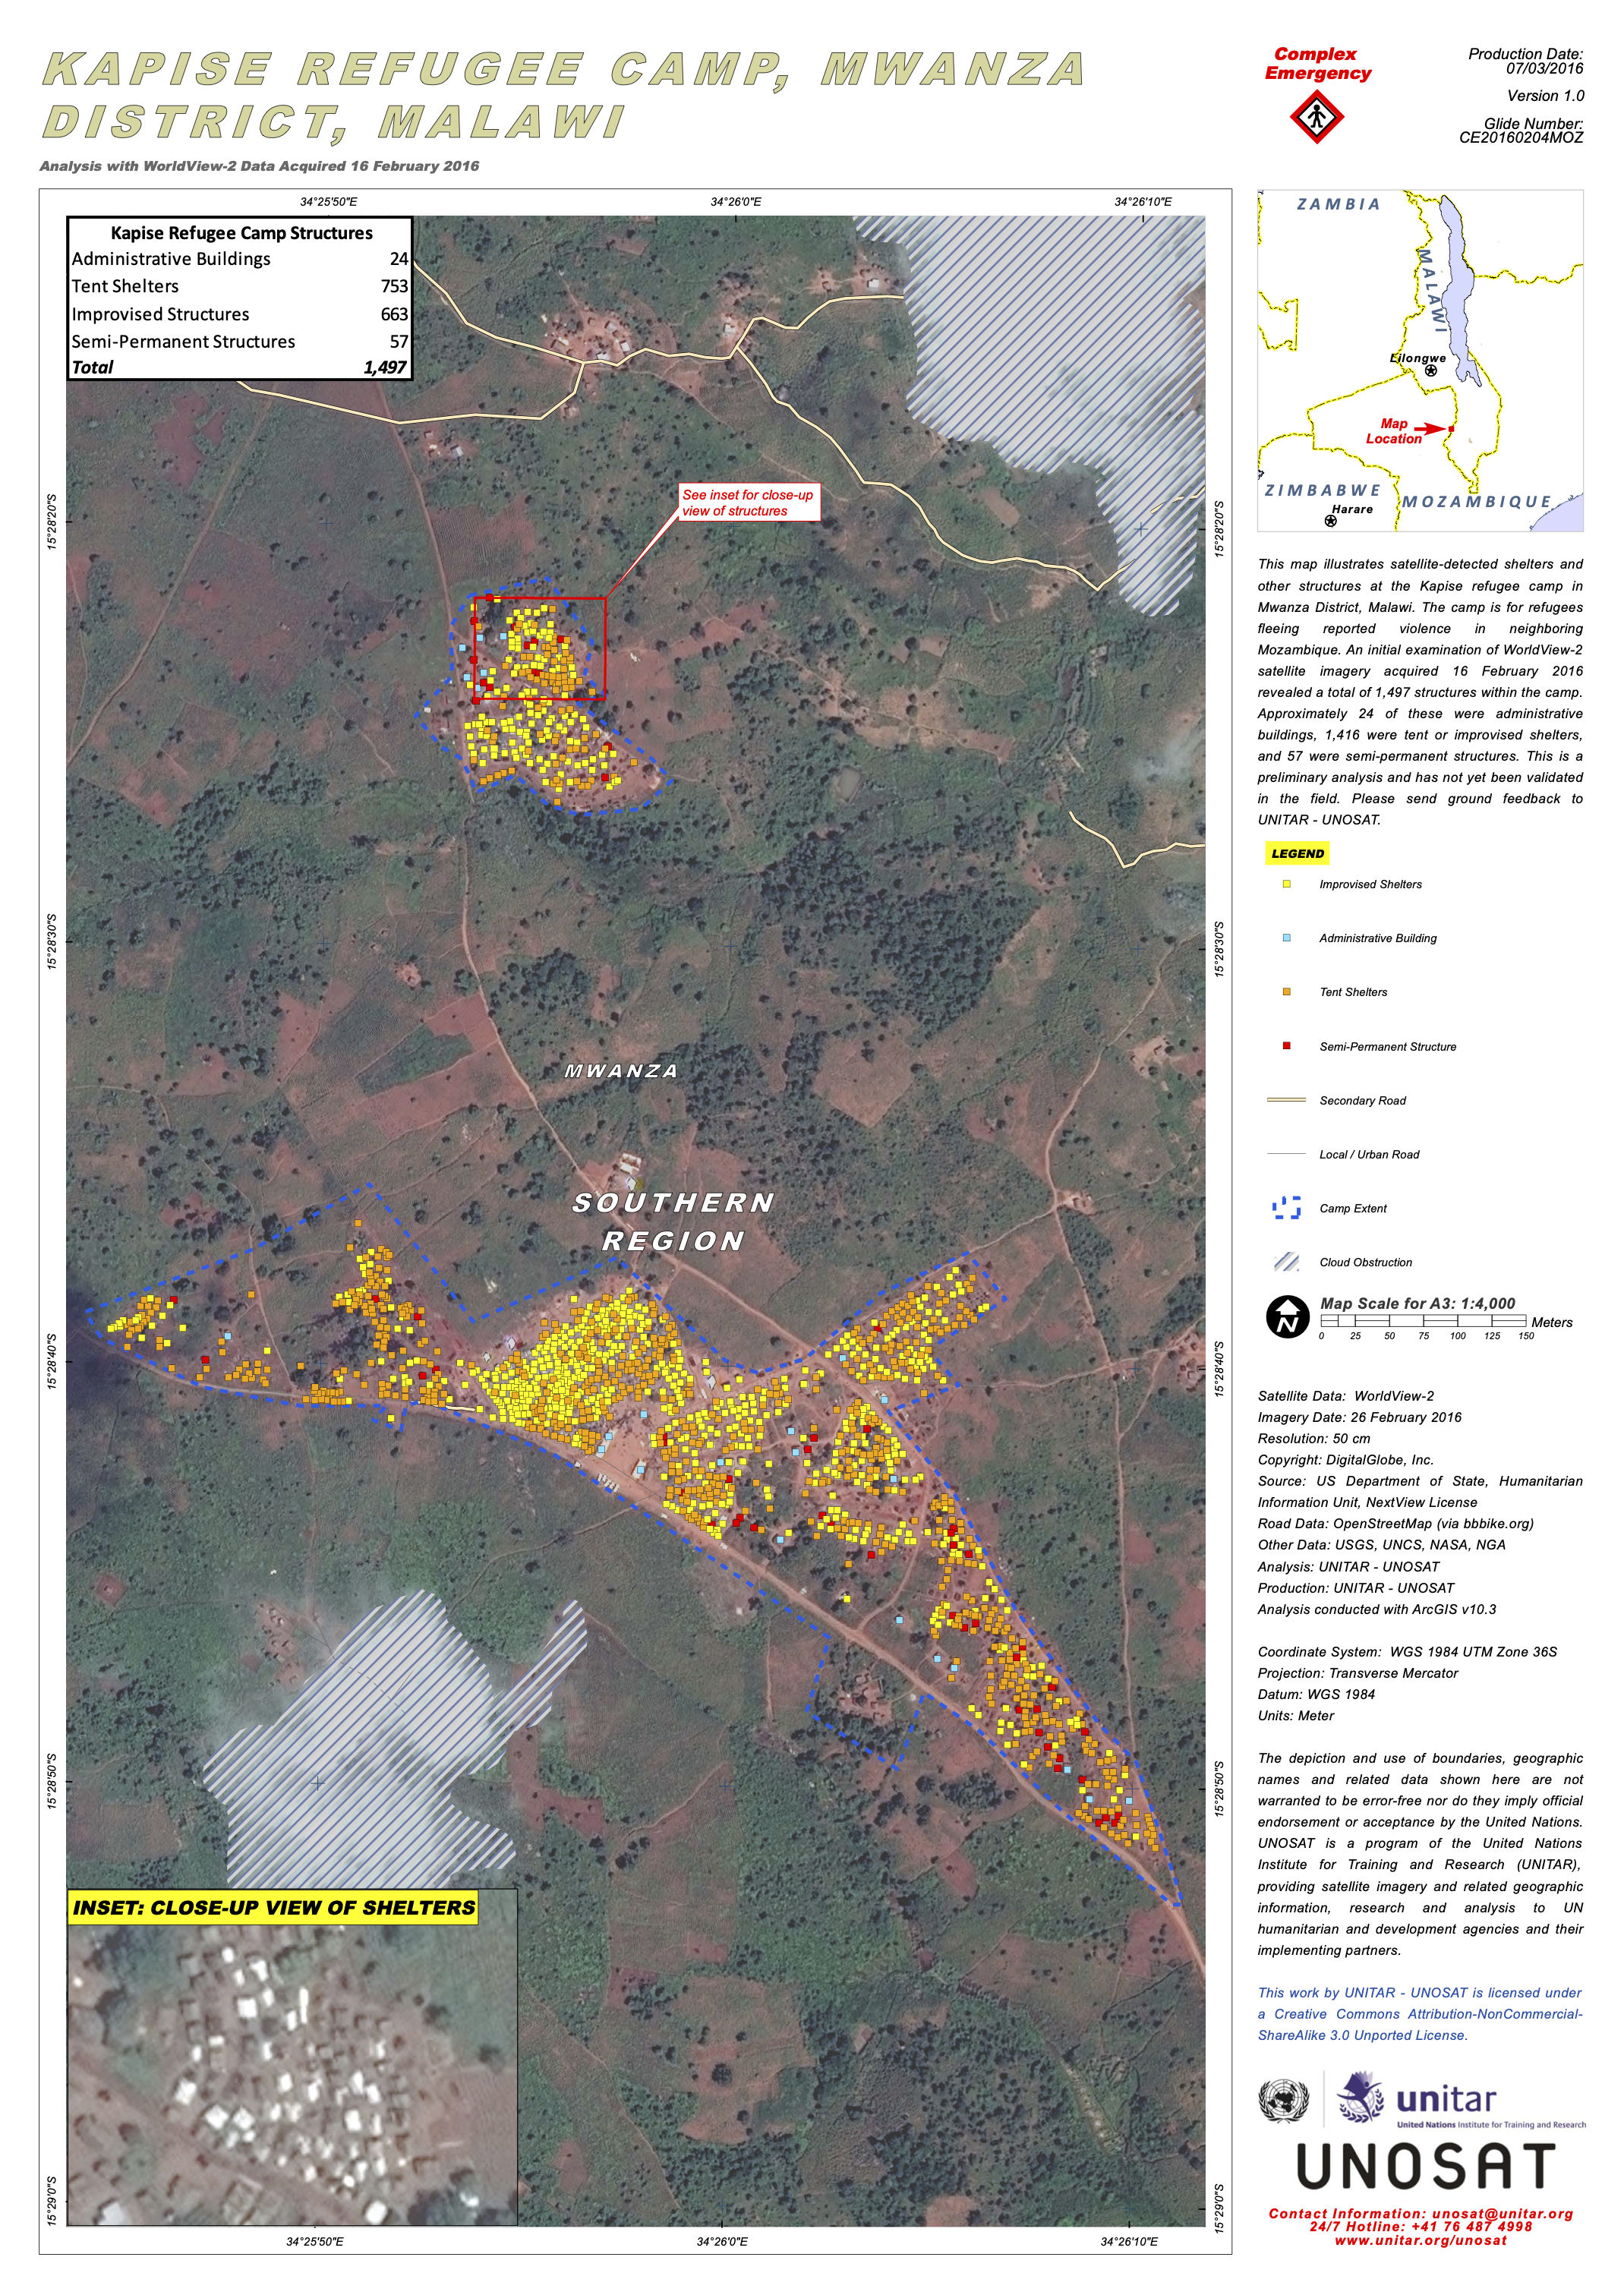
\includegraphics{part3/images/UNOSAT_A3_Potrait_Kapise_26Feb2016_v2.png}

}

}

\subcaption{\label{fig-unosat}Source: UNOSAT}
\end{minipage}%
%
\begin{minipage}[t]{0.50\linewidth}

{\centering 

\raisebox{-\height}{

\includegraphics{part3/images/Bakasi_camp_infrastructure_18052017_REACH.png}

}

}

\subcaption{\label{fig-reach}Source: REACH Initiative}
\end{minipage}%

\caption{\label{fig-examples}\textbf{Examples of Site maps}}

\end{figure}

\hypertarget{working-in-gis}{%
\section{Working in GIS}\label{working-in-gis}}

GIS software can open different file types: Vector files (which use
points, line segments and polygon objects to identify geographic
information), Raster files/images (which use cells/ pixels to represent
geographic information), and Delimited text files (such as .csv file
types). For example:

\begin{longtable}[]{@{}ll@{}}
\toprule()
Data Layer Example & File Type \\
\midrule()
\endhead
Aerial Imagery & Raster file \\
Location of healthcare facilities or service providers & Vector file \\
Population per block & Delimited Text file \\
\bottomrule()
\end{longtable}

\hypertarget{loading-data-layers-and-veryfying-projections}{%
\subsection{Loading data layers and veryfying
projections}\label{loading-data-layers-and-veryfying-projections}}

To prepare the site map,
\href{https://docs.qgis.org/2.8/en/docs/user_manual/working_with_vector/editing_geometry_attributes.html\#digitizing-an-existing-layer}{load
the data layers} into a GIS workspace, such as QGIS.

Most publicly available geographic information datasets are projected in
a world Coordinate Reference System (CRS) (WGS 84). When loading a layer
projected in a whole world CRS, the layer will look slightly distorted
in the workspace. Ensure that the
\href{https://docs.qgis.org/3.22/en/docs/user_manual/working_with_projections/working_with_projections.html\#project-coordinate-reference-systems}{Project
CRS} is set to the area of your site location. You can use the
\href{https://epsg.io/}{epsg.io} database of coordinate systems to know
the coordinate system you should be using for you context. All loaded
data layers need to be checked and
\href{https://docs.qgis.org/3.22/en/docs/user_manual/working_with_projections/working_with_projections.html\#layer-coordinate-reference-systems}{projected}
where needed, according to the project CRS.

\hypertarget{layers-and-elements-of-a-site-map}{%
\subsection{Layers and elements of a site
map}\label{layers-and-elements-of-a-site-map}}

This guide is accompanied by a site map template which can be loaded
into QGIS's Print Composer. Below is a dummy example of a site map
produced using this template.

\begin{figure*}

{\centering 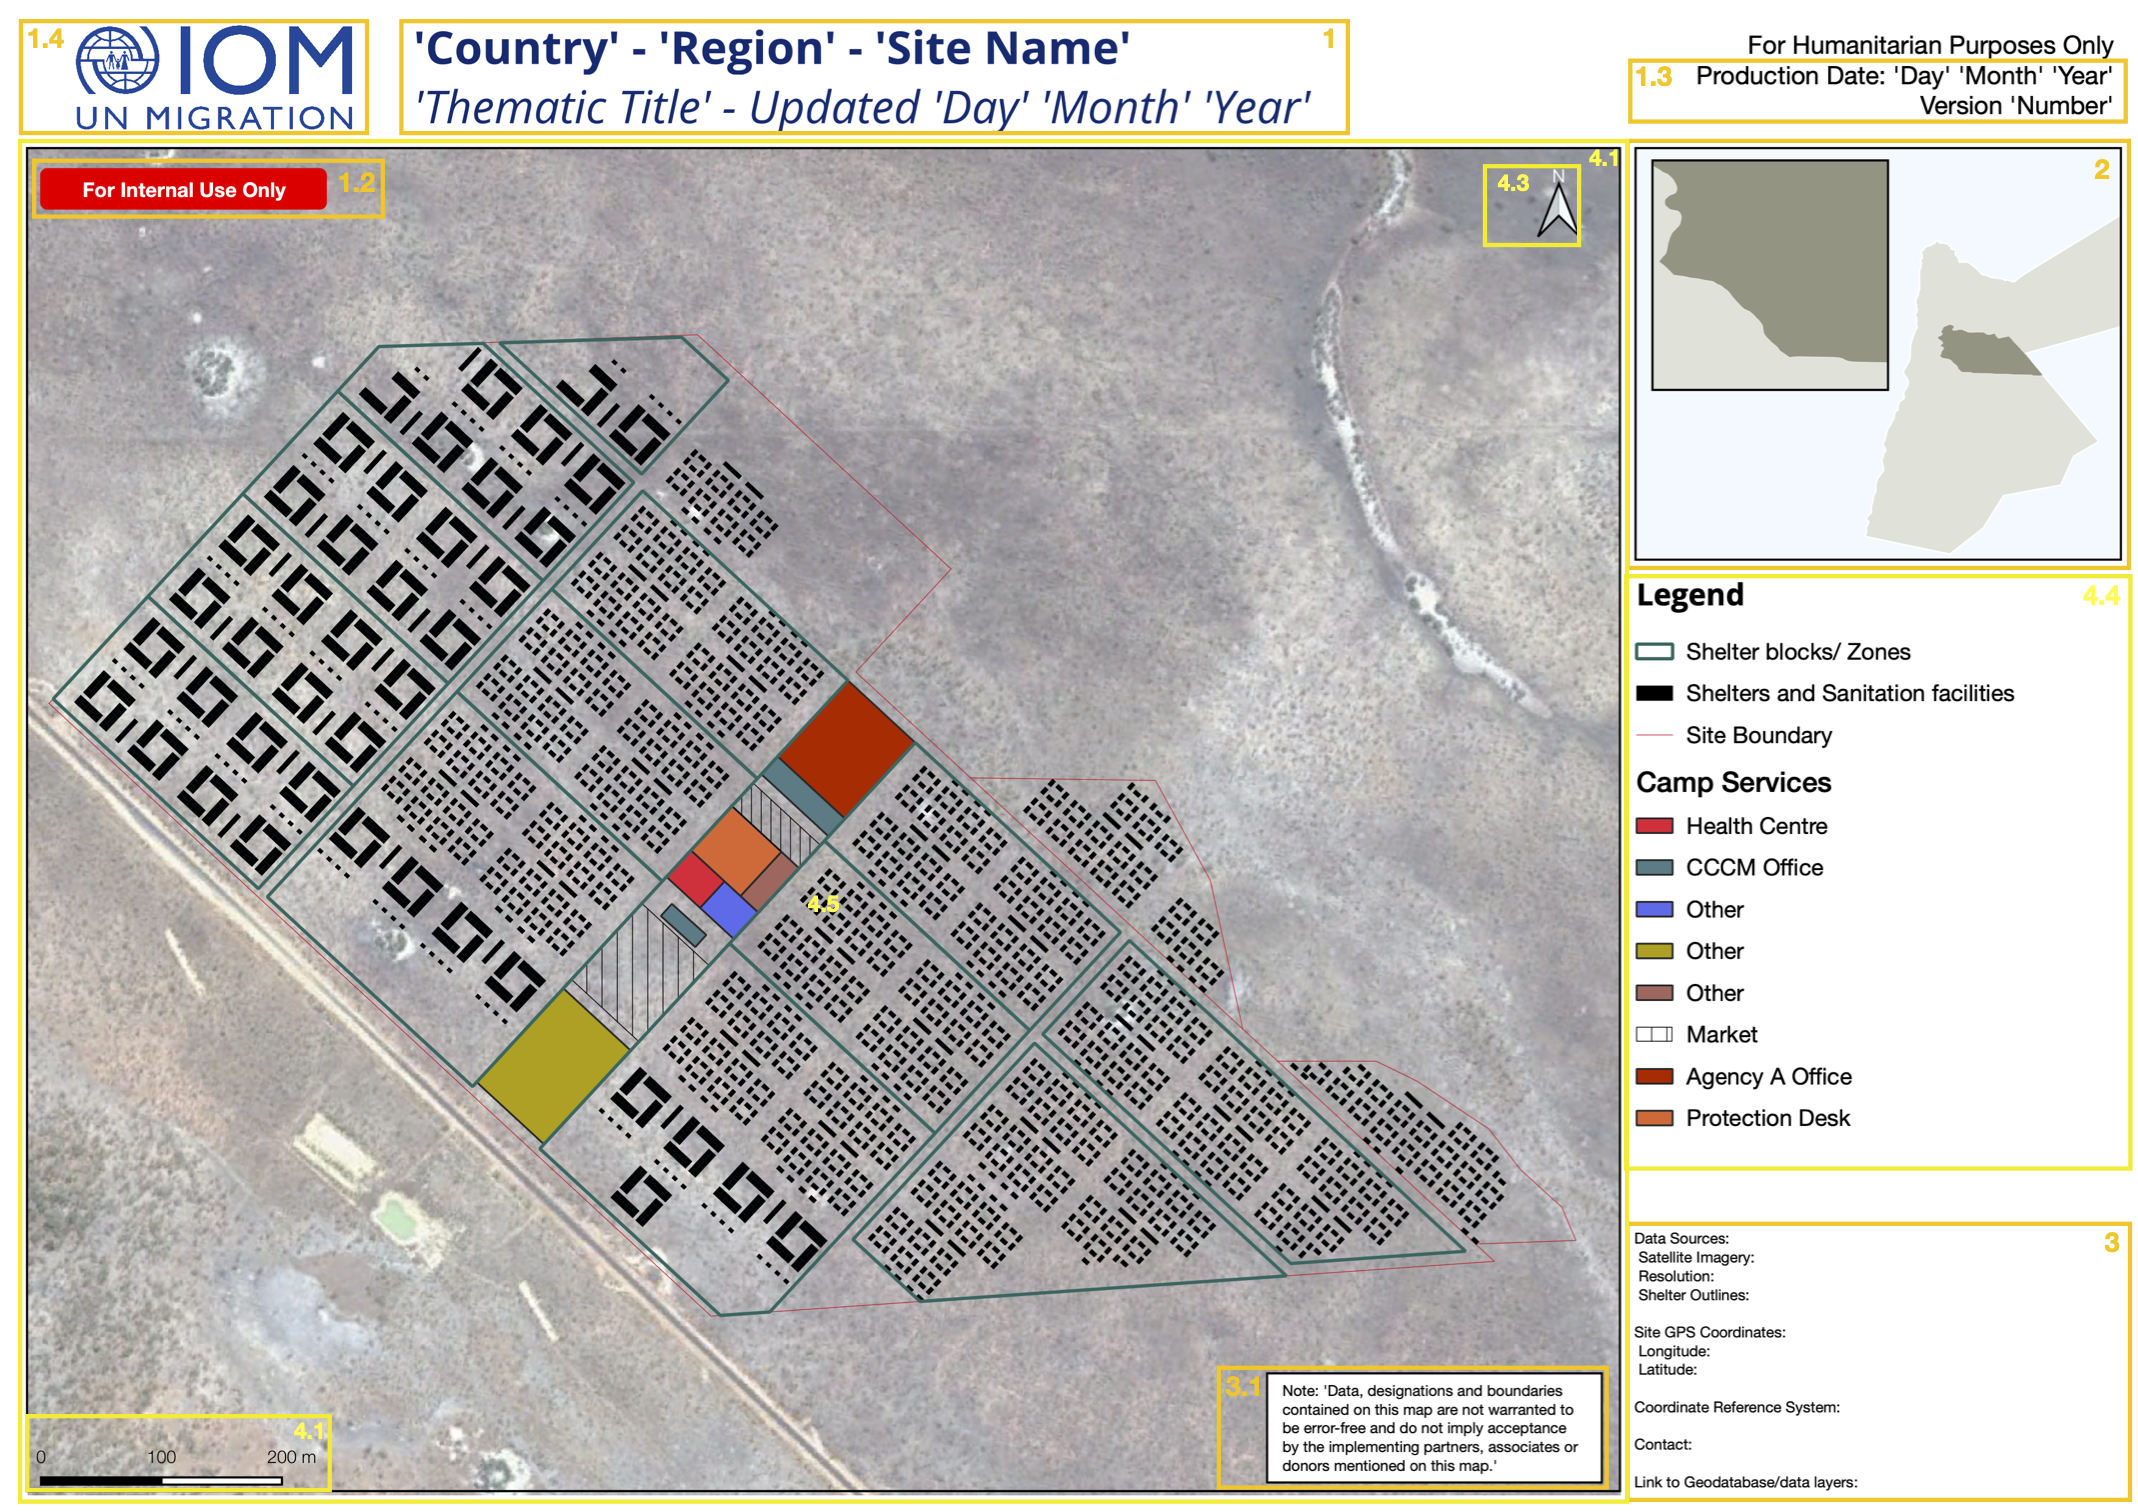
\includegraphics[width=0.91\textwidth,height=\textheight]{part3/images/dummy_site_map.png}

}

\caption{An example of a dummy site map composed in QGIS using the site
map template included in this guide. \emph{Source: IOM}}

\end{figure*}

\begin{tcolorbox}[enhanced jigsaw, opacitybacktitle=0.6, colbacktitle=quarto-callout-note-color!10!white, breakable, coltitle=black, title=\textcolor{quarto-callout-note-color}{\faInfo}\hspace{0.5em}{Note}, toprule=.15mm, bottomrule=.15mm, colback=white, left=2mm, toptitle=1mm, bottomtitle=1mm, arc=.35mm, colframe=quarto-callout-note-color-frame, titlerule=0mm, opacityback=0, rightrule=.15mm, leftrule=.75mm]

For the purposes of supporting a \textbf{standardized approach to the
production of static site maps}, and ensuring new \textbf{site maps can
be compared and used alongside existing maps}, the template provided in
this Site Mapping Guide is one approach to laying out a site map,
however this can and should be adapted based on the context and it's
audience.

\end{tcolorbox}

The following list of layers and elements can be included in the final
output:

\begin{itemize}
\item
  \textbf{Title and Subtitle} \textbf{(1)}

  \begin{itemize}
  \tightlist
  \item
    Country
  \item
    State
  \item
    Site Name
  \item
    Thematic Title
  \item
    Date site map was last updated
  \end{itemize}
\item
  Site map audience/ permission/ sharing restrictions \textbf{(1.2)}
\item
  Production date and version number of site map \textbf{(1.3)}
\item
  Agency/ NGO Logos \textbf{(1.4)}
\item
  \textbf{Inset maps} \textbf{(2)}

  \begin{itemize}
  \tightlist
  \item
    At Country/ Regional level
  \item
    At Regional/ Area level
  \end{itemize}
\item
  \textbf{Notes} \textbf{(3)}

  \begin{itemize}
  \tightlist
  \item
    Data sources
  \item
    Satellite Imagery source
  \item
    Imagery Resolution
  \item
    Coordinate system
  \item
    Site GPS coordinate points
  \item
    Agency/ NGO Logo
  \item
    Contact
  \item
    Link to Geodatabase/ corresponding data layers
  \item
    Disclose limitations regarding accuracy of site map \textbf{(3.1)}
  \end{itemize}
\item
  \textbf{Map}

  \begin{itemize}
  \tightlist
  \item
    Base Map (satellite/ aerial imagery) \textbf{(4.1)}
  \item
    Scale bar \textbf{(4.2)}
  \item
    Orientation indicators \textbf{(4.3)}
  \item
    Legend \textbf{(4.4)}
  \item
    Camp Infrastructure \textbf{(4.5)} :

    \begin{itemize}
    \tightlist
    \item
      Shelters
    \item
      Shelter blocks
    \item
      Zones
    \item
      WASH facilities
    \item
      Water points
    \item
      Education facilities
    \item
      Health Facilities
    \item
      Distribution points (Food/ NFI)
    \item
      Markets(s)
    \item
      Information desks
    \item
      CFM desks
    \item
      Other camp facilities
    \item
      Movement network (Roads, pathways)
    \item
      Community areas/ centre
    \item
      Religious buildings/ spaces
    \item
      Site Entrance(s)
    \item
      Site boundary
    \item
      Security facilities or guard points
    \item
      Fences/ Camp Boundaries
    \end{itemize}
  \end{itemize}
\item
  \textbf{Environment}

  \begin{itemize}
  \tightlist
  \item
    Host community
  \item
    Green belt
  \item
    Trees/ Vegetation
  \item
    Agricultural land
  \end{itemize}
\item
  \textbf{Optional additional labels}:

  \begin{itemize}
  \tightlist
  \item
    Functioning/ non-functioning facilities
  \item
    Male/ female latrines
  \item
    Unusable area
  \item
    Summary information/ figures

    \begin{itemize}
    \tightlist
    \item
      Site population (households and individuals)
    \item
      Site area
    \item
      Total no. of shelters
    \item
      Shelter type and size
    \item
      Quantity of sanitation blocks/ latrines/ showers
    \item
      Type of water supply
    \item
      Total no. of water points
    \end{itemize}
  \end{itemize}
\end{itemize}

\hypertarget{visualizing-data-layers}{%
\subsection{Visualizing data layers}\label{visualizing-data-layers}}

Once the files are opened in QGIS, they will appear as layers. These
layers can be duplicated in order to
\href{https://docs.qgis.org/3.22/en/docs/user_manual/style_library/symbol_selector.html\#the-symbol-selector}{show
different visualisations} of the same file.

\hypertarget{adding-fields-and-editing-attributes}{%
\subsection{Adding fields and editing
attributes}\label{adding-fields-and-editing-attributes}}

Shapefiles (ESRI Shapefile format) are the most common type of vector
file. This file format dataset consists of several files. Of these
different files, there are two which you should be familiar with for the
purposes of this site mapping exercise. First, the .shp file, which
contains the geometries of the features in the layer and secondly, the
.dbf file, which contains the feature \textbf{attributes}.

The attribute table interface allows you to view and {[}edit the
attribute data{]}
(https://docs.qgis.org/3.22/en/docs/user\_manual/working\_with\_vector/attribute\_table.html\#editing-attribute-values)
as well as
\href{https://docs.qgis.org/3.22/en/docs/user_manual/working_with_vector/attribute_table.html\#interacting-with-features-in-an-attribute-table}{interact
with features} in a layer (by selecting or filtering features for
example). Fields are columns of attribute values and these can be added,
deleted and edited through this interface.

\begin{tcolorbox}[enhanced jigsaw, opacitybacktitle=0.6, colbacktitle=quarto-callout-warning-color!10!white, breakable, coltitle=black, title=\textcolor{quarto-callout-warning-color}{\faExclamationTriangle}\hspace{0.5em}{Warning}, toprule=.15mm, bottomrule=.15mm, colback=white, left=2mm, toptitle=1mm, bottomtitle=1mm, arc=.35mm, colframe=quarto-callout-warning-color-frame, titlerule=0mm, opacityback=0, rightrule=.15mm, leftrule=.75mm]

Any saved changes made to a data layer in QGIS will also change the
source file. If you wish to edit/ delete or add features or attribute
values to a layer but do not want to edit the original source file,
\href{https://docs.qgis.org/2.8/en/docs/user_manual/working_with_vector/editing_geometry_attributes.html\#digitizing-an-existing-layer}{save
the layer as a separate file} \textbf{before} making your edits.
Additionally, removing a layer will remove it from the work space but
will not delete it from your source folder.

\end{tcolorbox}

\hypertarget{print-layouts-and-using-templates}{%
\subsection{Print Layouts and Using
Templates}\label{print-layouts-and-using-templates}}

With QGIS's layout composer, you can
\href{https://docs.qgis.org/3.22/en/docs/user_manual/print_composer/overview_composer.html\#the-layout-manager}{create
layouts} or use existing layout templates. The template file can be
downloaded \href{add\%20link}{here}. Once the layout is complete,
\href{https://docs.qgis.org/3.22/en/docs/user_manual/print_composer/create_output.html}{save
and export the print layout} as an image, an svg (for future editing in
other software such as Adobe Illustrator or InkScape, select
\href{https://docs.qgis.org/3.22/en/docs/user_manual/print_composer/overview_composer.html\#layout-export-settings}{export
as vectors}), or as a PDF. If saving as a PDF, consider saving the
layout as a GeoPDF by selecting 'Create Geospatial PDF (GeoPDF) in the
export PDF settings (refer to
\href{https://sitemapping.guide/part3/collaboration.html}{Section 7:
Collaboration} for why you should export your site map alsp as a
GeoPDFs)

\hypertarget{saving-the-data-layers-and-styles-into-a-geopackage}{%
\subsection{Saving the data layers and styles into a
Geopackage}\label{saving-the-data-layers-and-styles-into-a-geopackage}}

Data layers are saved on your local computer. To facilitate sharing
geographic information, data layers can be compressed into a
\href{https://docs.qgis.org/3.22/en/docs/user_manual/managing_data_source/supported_data.html?highlight=fields\%20attributes\#geopackage}{\textbf{Geopackage}}.
The QGIS project and all the data used in the project can be saved using
the
\href{https://www.cadlinecommunity.co.uk/hc/en-us/articles/4403555255697-QGIS-Package-Layers}{Package
Layers tool} and easily shared and stored as such for future use.

\hypertarget{collaboration}{%
\chapter{Collaboration}\label{collaboration}}

Throughout the development cycle of site maps, the contributions and
participation of the different stakeholders identified earlier in this
guide, is key to producing high quality, updated site maps. Static PDF
site maps are the main output of this workflow. However, it is also
important to recognise that other products are created in the process of
making these maps, such as:

\begin{itemize}
\tightlist
\item
  Aerial/ Satellite imagery of sites in which CCCM, shelter or other
  humanitarian activities are being carried out,
\item
  The geopackage which contains geographic information and data layers
  of the site infrastructure,
\item
  GeoPDFs,
\item
  Site map template
\end{itemize}

\hypertarget{information-and-knowledge-management}{%
\section{Information and knowledge
management}\label{information-and-knowledge-management}}

These are valuable information products which can be used by colleagues
and other humanitarian actors to conduct thematic analysis as well as
serve as an evidence base for advocacy, planning and decision making.
More importantly, these products are tools to collaborate with
stakeholders and actors on the ground that in turn can:

\begin{enumerate}
\def\labelenumi{\arabic{enumi}.}
\tightlist
\item
  Verify and validate the information,
\item
  Feedback and suggest modifications,
\item
  Update the data when changes occur on the ground.
\end{enumerate}

Therefore, the manner in which this data is stored, presented and shared
is crucial to both allow for and promote the use of site maps.

\begin{tcolorbox}[enhanced jigsaw, opacitybacktitle=0.6, colbacktitle=quarto-callout-note-color!10!white, breakable, coltitle=black, title=\textcolor{quarto-callout-note-color}{\faInfo}\hspace{0.5em}{Note}, toprule=.15mm, bottomrule=.15mm, colback=white, left=2mm, toptitle=1mm, bottomtitle=1mm, arc=.35mm, colframe=quarto-callout-note-color-frame, titlerule=0mm, opacityback=0, rightrule=.15mm, leftrule=.75mm]

IOM and partner agency/ NGO staff can and are encouraged to share these
data products with the CCCM Global Cluster so there is continuity in the
management of site data. The CCCM Global cluster can play a role in
facilitating the storage, dissemination and use of site data whilst
ensuring it is done so responsibly.

\end{tcolorbox}

\hypertarget{generating-reading-and-annotating-geopdfs}{%
\section{Generating, reading and annotating
geoPDFs}\label{generating-reading-and-annotating-geopdfs}}

In the previous section, we looked at exporting print layouts as
GeoPDFs. GeoPDFs are PDFs with embedded georeferenced location
information.

GeoPDFs can be imported into
\href{https://www.avenzamaps.com/mobile-maps?campaignid=10221828697\&adgroupid=102940455500\&adid=453328850375\&gclid=Cj0KCQiAg_KbBhDLARIsANx7wAxTp38Kmz11Ou-eCXzYSF_EkQpvBq3PvAo3sxuIS88hZMkaglVMWSAaAtEFEALw_wcB}{Avenza
maps}. The app uses the built in GPS in a tablet or smartphone to locate
users when out of range of a network or internet connection. Users can
mark points of interest, attach photos with exact location, and add
annotations to existing features.

\hypertarget{gathering-feedback-and-map-iterations}{%
\section{Gathering feedback and map
iterations}\label{gathering-feedback-and-map-iterations}}

Through Focus group discussions and site walks, the site maps can be
annotated by different stakeholders to mark for example, errors in the
map, changes in the layout of the site, the location of new or closed
services etc. The site map can either be project or printed in large
formats or imported in Avenza map to be used during site walks in order
to determine the precise location of different features.

\hypertarget{using-site-maps-in-practice}{%
\section{Using Site maps in
Practice}\label{using-site-maps-in-practice}}

Site maps can provide a spatial perspective on issues and risks within
sites. They can be used as inputs to safety audits, identification of
risk factors and support coordinated planning and coordination of
response activities.

\part{Annexes}

\hypertarget{acknowledgements}{%
\chapter*{Acknowledgements}\label{acknowledgements}}
\addcontentsline{toc}{chapter}{Acknowledgements}

\markboth{Acknowledgements}{Acknowledgements}

We would like to thank the following people for their support during all
stages of the development of this guidance:

\hypertarget{glossary}{%
\chapter*{Glossary}\label{glossary}}
\addcontentsline{toc}{chapter}{Glossary}

\markboth{Glossary}{Glossary}

A glossary of terms used throughout this guide:

\begin{description}
\tightlist
\item[DSM]
Digital Surface Model. A modelling of a an area that include foliage and
structures.
\item[DTM]
Digital Terrrain Model. Similar to DSM but excluding foliagge and other
structures. Also Displacement Tracking Matrix, an IOM initiative that
gathers data on mobility, vulnerability and needs.
\item[Drone]
Common term for unmanned or remotely-piloted aircraft.
\item[Georeferencing]
The act of aligning geographic data (such as a map) to a known
coordinate system.
\item[GIS]
Geographic information system. In general terms, a system that is
designed to manipulate, store, analyze, and manage spatial and
geographic data.
\item[GSD]
Ground sample distance. The resolution of an aerial image
\item[IOM]
International Organization for Migration.
\item[Nadir]
In aerial photography, the point on the ground that lies directly below
the perspective center of the camera lens; also, images taken from this
perspective (i.e., straight down).
\item[Orthomosaic]
A two-part process in which a number of images are combined together or
``stitched'' into a single image and also corrected for distortion.
\item[Orthorectification]
A process of removing the efects of image perspective and relief efects
by using camera model information and elevation data, creating a fnal
image that has a constant scale.
\item[RTK]
Real time kinematic. A technique used to extract
more-precise-than-normal position data from global satellite navigation
timing signals.
\item[UAV]
Unmanned Aerial Vehicle, commonly known as a drone. Radio controlled
fixed-wing or rotorcraft.
\end{description}

\hypertarget{further-reading}{%
\chapter*{Further reading}\label{further-reading}}
\addcontentsline{toc}{chapter}{Further reading}

\markboth{Further reading}{Further reading}

\hypertarget{refs}{}
\begin{CSLReferences}{0}{0}
\end{CSLReferences}

\href{http://drones.newamerica.org/primer/}{DRONES AND AERIAL
OBSERVATION: New Technologies for Property Rights, Human Rights, and
Global Development}

\href{https://unicef.github.io/drone-4sdgtoolkit/}{UNICEF Drones for
Sustainable Development Goals Toolkit}

\href{https://uav-guidelines.openaerialmap.org/}{HOT OSM UAV Mapping
Guidelines}

\href{https://interagencystandingcommittee.org/operational-response/iasc-operational-guidance-data-responsibility-humanitarian-action\#:~:text=Data\%20responsibility\%20in\%20humanitarian\%20action\%20is\%20the\%20safe\%2C\%20ethical\%20and,and\%20the\%20stakes\%20are\%20high.}{IASC
Operational Guidance on Data Responsibility in Humanitarian Guidance}

\href{https://www.icrc.org/en/data-protection-humanitarian-action-handbook}{ICRC
Handbook on Data Protection in Humanitarian Action}


\backmatter

\end{document}
